In this section, we derive an adaptive implementation scheme for real-time controllers to address the problems discussed in Section~\ref{sec:problem-form}.
We explain the intuition behind the proposed adaptation; then, starting from an arbitrary linear control algorithm, we show how to derive the adapted controller.
The adaptive controller is complemented with a probabilistic analysis method to evaluate its effectiveness for a given control system and a given deadline miss model.

\subsection{Adaptive Controller Synthesis}%
\label{sec:adaptation}%
%
To simplify and generalise the adaptation approach, we do not assume any information about the control design, apart from the controller itself. 
In practice, this implies that we consider neither the specific control design technique, the control system requirements, nor the plant's dynamics.
The controller is assumed to be given in state-space form, specified by~\eqref{eq:ctrler}.
This assumption is made without loss of generality, since any realisable linear digital controller can be expressed in this form~\cite{Astrom:2008}.

%ideal controller
The controller behaves \emph{ideally} when every control period includes one job completing the execution of Equation~\eqref{eq:ctrler}, i.e., every job hits its deadline.
By iterating the equation, the desired controller state and control action at any future time step can be computed. 
We formally define this behaviour as follows:

\begin{definition}[Ideal Controller]%
    We denote the \emph{ideal controller}, $\ctrler\funof{\counter}$, as the discrete-time LTI controller $\ctrler$ evolved over an interval of $\counter+1$ consecutive deadline hits.
    The controller state and output at the end of the interval are
    \begin{equation}
        \label{eq:ctrler-ideal}
        \ctrler\funof{\counter}:\,\, 
        \left\{\begin{aligned}
            z_{t+\counter+1} &= \Ac^{\counter+1}\,z_{t} + \textstyle\sum_{i=0}^{\counter} \Ac^i \Bc \,y_{t+\counter-i}\\
            u_{t+q+1} &= \Cc\, \Ac^{q}\,\,z_t + \\
            &\hspace{-2em}+ \Cc\, \textstyle\sum\nolimits_{i=1}^{q}\, \left[ \Ac^{i-1}\, \Bc\, y_{t+q-i}\right] 
            + \Dc\, y_{t+q}.
        \end{aligned}\right.
    \end{equation}
\end{definition}
With $\counter=0$ we obtain the ideal controller behaviour over a single time step.

From the definition above, we see how the quantities of interest, $z$ and $u$, are computed using the values of $y$ in the interval $\left[ t, t+\counter \right]$. 
These values correspond to the periodic measurements coming from the sensors.
%
In the presence of deadline misses, the control task discards the measurements and does not update the controller's state.
Thus, both the state and output of the controller deviate from their desired behaviours. 
Applying Equation~\eqref{eq:ctrler} to a scenario of $\counter$ consecutive deadline misses, we obtain the following:

\begin{definition}[Nominal Controller]%
    We denote the \emph{nominal controller}, $\ctrler^n\funof{\counter}$, as the discrete-time LTI controller $\ctrler$ evolved over an interval of $\counter$ consecutive deadline misses followed by one deadline hit. 
    After the hit, the state and output are given by
    \begin{equation}
        \label{eq:ctrler-miss}
        \ctrler^n\funof{\counter}:\,\, 
        \left\{\begin{aligned}
            z_{t+\counter+1} &= \Ac\,z_{t} + \Bc\,y_{t+\counter}\\
            u_{t+\counter+1} &= \Cc\,z_{t} + \Dc\,y_{t+\counter}.
        \end{aligned}\right.
    \end{equation}
    In the absence of deadline misses, we have $\ctrler^n\funof{0} = \ctrler$.
\end{definition}

By comparing \eqref{eq:ctrler-ideal} and~\eqref{eq:ctrler-miss} we see that, when deadline misses occur, the controller state $z_{t+\counter+1}$ and control action $u_{t+\counter+1}$ diverge from the ideal values, i.e., the ones that would be obtained in the presence of only deadline hits. 
To compensate for this error (and consequently minimise it), we propose to dynamically alter the controller's computations in real time according to the number of deadline misses. 

Ideally, we would like an adaptive controller $\ctrler^a\funof{\counter}$ that mimics the ideal controller $\ctrler\funof{\counter}$ for any $\counter$.
However, this is infeasible due to how the controller's dynamics evolves during an interval of deadline misses.
More specifically, Equation~\eqref{eq:ctrler-ideal} shows that $\ctrler\funof{\counter}$ depends on the values of $y_{t+i}$ for $i \in \left\{ 0, 1, \ldots, \counter-1 \right\}$.
When the control task is subjected to faults, the corresponding jobs $j_{t+i}$ miss their respective deadline. 
Thus, the unfinished jobs are terminated prematurely, a new job is released, and the corresponding measurement values $y_{t+i}$ are lost.
The nominal controller, after a series of misses, has access only to the sample $y_{t+\counter}$.
This fundamentally limits how well the controller's ideal behaviour can be reconstructed.

Hence, we propose the use of an interpolation scheme to minimise the effect of the lost measurement values.
We approximate the missing measurement values using a linear interpolation between $y_{t-1}$ and $y_{t+\counter}$ according to
%
\begin{equation}
    \label{eq:interpolation}
    \hat y_{t+\counter-i} = \frac{i\, y_{t-1} + (\counter+1-i)\, y_{t+\counter}}{\counter+1} .
\end{equation}
%
If we substitute the values of $y$ that are missing in the ideal controller, Equation~\eqref{eq:ctrler-ideal}, with the corresponding interpolated ones $\hat y$ from Equation~\eqref{eq:interpolation}, we obtain an adaptive controller as follows:

\begin{definition}[Adaptive Controller]%
    We denote the \emph{adaptive controller}, $\ctrler^a\funof{\counter}$, as an adaptation of the controller $\ctrler$ evolved over an interval of $\counter$ consecutive deadline misses followed by one deadline hit.
    After the hit, the state and output are
    \begin{equation}
        \label{eq:adaptive}
        \ctrler^a\funof{\counter}: \,\,
        \left\{
            \begin{aligned}
                z_{t+\counter+1} &= F_z(\counter)\,z_{t} +  F_y(\counter)\,y_{t-1} + G_y(\counter)\,y_{t+\counter} \\
                u_{t+\counter+1} &= H_z(\counter)\,z_{t} + H_y(\counter)\,y_{t-1} + K_y(\counter)\,y_{t+\counter},
            \end{aligned}\right.
    \end{equation}
    where
    \begin{equation*}
        \begin{aligned}
            \Ac_z(\counter) &= \Ac^{\counter+1} \\
            \Ac_y(\counter) &= \textstyle\sum\nolimits_{i=0}^{\counter}\, \tfrac{i}{\counter+1}\, \Ac^{i}\, \Bc \\
            \Bc_y(\counter) &= \textstyle\sum\nolimits_{i=0}^{\counter}\, \tfrac{\counter+1-i}{\counter+1}\, \Ac^{i}\, \Bc \\
            \Cc_z(\counter) &= \Cc\, \Ac^\counter \\
            \Cc_y(\counter) &= \Cc\, \textstyle\sum\nolimits_{i=1}^{\counter}\, \tfrac{i}{\counter+1}\, \Ac^{i-1}\, \Bc \\
            \Dc_y(\counter) &= \Dc + \Cc\, \textstyle\sum\nolimits_{i=1}^{\counter}\, \tfrac{\counter+1-i}{\counter+1}\, \Ac^{i-1}\, \Bc.
        \end{aligned}
    \end{equation*}
\end{definition}
Note that for $\counter = 0$ we recover the original controller.

All matrices in $\ctrler^a\funof{q}$ ($\counter \in \{0, \ldots, \counter_{max}\}$) can be precomputed and stored in memory.
Compared to the nominal controller, the two matrices $F_y$ and $H_y$ of size $n_z \times n_y$ and $n_u \times n_y$ need to be added to the controller, and one full set of controller matrices needs to be stored for each value of $\counter$.
The memory requirement thus grows linearly with $\counter_{max}$.
%the number $\counter$ of maximum tolerated misses.
%This is exactly $\counter_{max}$ times the size of the non-adaptive controller expanded with $F_y$ and $H_y$.
The adaptive controller also needs to store the old measurement value $y_{t-1}$, which makes it marginally more complex.

% How we overcome the limitations of previous work
We now briefly discuss how the limitations described in Section~\ref{sec:problem-form} are addressed.
This work proposes an adaptation of the $\Ac$, $\Bc$, $\Cc$, and $\Dc$ matrices of the controller, thus adapting also the \emph{dynamic} part of the controller.
The adaptive controller's matrices can be precomputed directly from the specified controller using Equation~\eqref{eq:adaptive}, and then stored in memory for each $\counter \leq \counter_{max}$.
The control algorithm can be developed independently of this adaptation, hence no extra design effort is needed.
For $\counter=0$ the adaptive and the ideal controllers are equivalent, i.e., $\ctrler^a\funof{0} = \ctrler\funof{0}$, thus guaranteeing that the controller's performance is not degraded under ideal conditions.
Concerning the limitation of increased runtime overhead, each time a job is released, the counter $\counter$ of immediately preceding deadline misses is evaluated and the corresponding controller matrices are selected.
Hence, the execution time of the adaptive controller will be independent of $\counter$ and only marginally longer than for the nominal controller.

\begin{figure}[tp!]
    \centerline{\def \ada {\figdir/example-figs/adaptive.csv}
\def \lqg {\figdir/example-figs/lqg.csv}
\def \nom {\figdir/example-figs/lqg-nominal.csv}

\begin{tikzpicture}
    \footnotesize

    %Main axes
    \begin{axis}[%
            height=\timeplotheight,
            width=\columnwidth,
            xmin=0,
            xmax=5,
            ymin=-0.4,
            ymax=1.1,
            xlabel={Time (s)}, 
            ylabel={State},
            ytick={-0.4,-0.2,0,0.2,0.4,0.6,0.8,1.0,1.2},
            yticklabels={-0.4,-0.2,0,0.2,0.4,0.6,0.8,1.0,1.2},
            ylabel near ticks,
            grid=major,
            grid style={dashed,black!20},
            legend cell align=left,
            scatter/classes={a={mark=x, mark size=3, color=misscolour}},
            % legend columns = 2
            ]
        
        % LQG x
        \addplot[lqgnomcolour, solid, very thick] table[x=T, y=X, col sep=comma] {\nom};
        
        % LQG x
        \addplot[lqgcolour, dash pattern={on 7pt off 2pt}, very thick] table[x=T, y=X, col sep=comma] {\lqg};
        
        % Ada x
        \addplot[adacolour, dash pattern={on 7pt off 2pt}, very thick] table[x=T, y=X, col sep=comma] {\ada};
        
        % Misses
        % scatter src=explicit symbolic gets the scatter definition in axis options.
        \addplot+[scatter, only marks, scatter src=explicit symbolic] coordinates{
            (0.3, -0.4) [a]
            (0.7, -0.4) [a]
            (0.9, -0.4) [a]
            (1.6, -0.4) [a]
            (2.1, -0.4) [a]
            (2.2, -0.4) [a]
            (2.3, -0.4) [a]
            (2.9, -0.4) [a]
            (3.2, -0.4) [a]
            (3.5, -0.4) [a]
            (3.8, -0.4) [a]
            (4.1, -0.4) [a]
            (5.0, -0.4) [a]
        };
        
        % Legend
        \legend{$x_2$ ($\ctrler_2$ -- ideal), $x_2$ ($\ctrler^n_2$ -- nominal), $x_2$ ($\ctrler^a_2$ -- adaptive), Overrun};
    \end{axis}

\end{tikzpicture}
}
    \caption{The state $x_2$ corresponding to $\plant$ being controlled by the LQG controller $\ctrler_2$ (dashed green) or adaptive LQG (dashed orange) controller during an interval of sporadic overloads ($\times$).
    The corresponding ideal behaviour (system not subject to overruns, solid green) is also plotted.}
    \label{fig:lqgs-lqgd}
\end{figure}

In Section~\ref{sec:problem-form}, we presented a motivating example of why it is insufficient to analyse static controllers subject to overruns.
We conclude this section with a continuation of this example showing the benefits of our scheme.

\begin{example}[Application to Motivating Example]%
    Consider the plant $\plant$, from Equation~\eqref{eq:example-plant}, controlled by the LQG controller $\ctrler_2$.
    We apply our proposed scheme to $\ctrler_2$, obtaining the corresponding adaptive controller $\ctrler_2^a\funof{\counter}$.
    In Figure~\ref{fig:lqgs-lqgd}, we compare the plant state obtained by controlling the plant using the two controllers, subject to the same deadline misses as in Figure~\ref{fig:lqr-lqg}.
    The dashed green line and the dashed orange line correspond, respectively, to the nominal LQG (the same as in Figure~\ref{fig:lqr-lqg}) and adaptive LQG.
    The solid green line corresponds to the ideal controller's behaviour, i.e., in the absence of deadline misses.
    We note a significant improvement in the performance of the adaptive LQG compared to the nominal LQG: the oscillations disappear and the state converges faster.
\end{example}

The proposed adaptive controller is inspired by the ideal controller $\ctrler\funof{\counter}$, % not subjected to deadline misses.
but there is no a priori guarantee that it will perform better than the nominal controller $\ctrler^n\funof{\counter}$. 
However, for a given plant and deadline miss model, the closed-loop system can be analysed and compared for different controllers. 
Since the actual sequence of hits and misses is generally unpredictable, in the next section, we propose a probabilistic method to compare the performance of the adaptive controller with the nominal controller.

\subsection{Stochastic Performance Analysis}
\label{sec:analysis}
To analyse the performance of the closed-loop system, we need to model the plant, the external disturbance $w$, and the sequences of deadline misses.
For what concerns the plant, we consider the standard state-space model presented in Equation~\eqref{eq:plant}.
The plant disturbance $w$ and the sequence of deadline hits and misses are modelled as stationary random processes with known statistical properties.
This allows us to analyse the time-averaged performance of the closed-loop system subject to deadline misses.
The analysis offered here is inspired by~\cite{Nilsson:1998}, which in turn relies on classical results for jump linear systems~\cite{Blair:1975}.

The control performance is measured in terms of the weighted stationary variance of the plant output $y$,
\begin{equation}
    \label{eq:cost}
    J = \E{ y_t^{\T} Q y_t },
\end{equation}
where $Q \in \R^{n_y \times n_y}$ is a positive semidefinite weighting matrix\footnote{Without loss of generality, we assume that zero is the desired plant output. A non-zero reference value can be modelled as an exogenous signal that is stored in the plant and offset in the measurement signal.}.
A smaller value of the cost $J$ is better, as it means that the controller can suppress the disturbance $w$ more effectively.
Additionally, the closed loop is guaranteed to be \emph{stable} in the mean-square sense as long as $J$ is finite~\cite{Fang:2002}, i.e., $J < \infty$.

The state of the complete system consists of the plant and the controller in feedback interconnection, together with the buffered previous measurement value and the calculated next control signal.
Accordingly, we define the closed-loop state vector as
\begin{equation*}
    \tilde{x}_t = \begin{bmatrix} x_t \\ z_t \\ y_{t-1} \\ u_t \end{bmatrix} .
\end{equation*}
As seen in Figure~\ref{fig:ctrl-loop}, the only external input of the closed-loop system is the disturbance $w$.
Hence, the state of the closed loop evolves according to the time-varying linear system
\begin{equation}
    \label{eq:cl-system}
    \tilde{x}_{t+1} = \clmat{}_{t} \tilde{x}_t + \clinp{} w_t.
\end{equation}
Here,
\begin{equation*}
    \clinp{} = \begin{bmatrix} \Wp \\ 0_{(n_z+n_y+n_u) \times n_w} \end{bmatrix},
\end{equation*}
while $\clmat{}_t$ can be either $\clmat{}_{hit}(\counter)$ or $\clmat{}_{miss}$, depending on whether the current deadline was hit or missed, and defined as
\begin{equation*}
    \clmat{}_{hit}(\counter) = \begin{bmatrix} \Ap & 0 & 0 & \Bp \\
        \Bc_y(\counter) \, \Cp & \Ac_z(\counter) & \Ac_y(\counter) & \Bc_y(\counter) \, \Dp \\
        \Cp & 0 & 0 & \Dp \\
        \Dc_y(\counter) \, \Cp & \Cc_z(\counter) & \Cc_y(\counter) & \Dc_y(\counter) \, \Dp
    \end{bmatrix},
\end{equation*}
where $\counter$ denotes the number of consecutive deadline misses since the last hit, and
\begin{equation*}
    \clmat{}_{miss} = \begin{bmatrix} \Ap & 0 & 0 & \Bp \\
        0 & I_{n_z} & 0 & 0 \\
        0 & 0 & I_{n_y} & 0 \\
    0 & 0 & 0 & I_{n_u} \end{bmatrix}.
\end{equation*}

Assuming that $w$ is a zero-mean white noise process with known covariance matrix $R = \E{w_t \cdot w_t^{\T}} \in \R^{n_w \times n_w}$, we can calculate how the state covariance, $P_t = \E{\tilde{x}_t\cdot \tilde{x}_t^{\T}}$, evolves over time.
Evaluating the covariance of both sides in Equation~\eqref{eq:cl-system} we obtain (see, e.g., \cite{AstWit:1984})
\begin{equation}
    \label{eq:covariance}
    P_{t+1} = \clmat{}_t P_t \clmat{}_t^{\T} + \clinp{} R \clinp{}^{\T} .
\end{equation}

\begin{figure}[t]
    \centerline{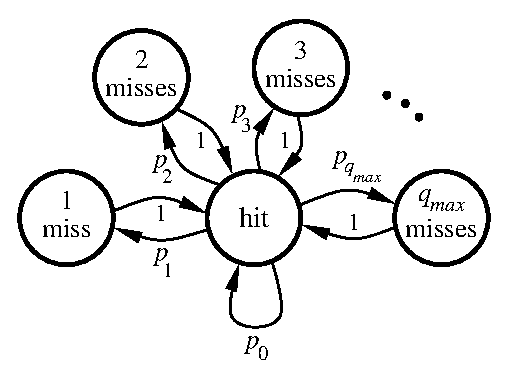
\includegraphics[scale=0.7]{\figdir/misses.eps}}
    \caption{Markov model for the random sequence of hits and misses.}
    \label{fig:Markov}
\end{figure}

We model the task execution as a random process, assuming that the pattern of hits and misses in the real-time system is described by the homogeneous Markov model shown in Figure~\ref{fig:Markov}.
In this model, after each hit, the system will experience a miss interval of length $\counter \in \{0,\ldots,\counter_{max}\}$ with independent probability $p_\counter$. Naturally, $\sum_{i=0}^{\counter_{max}} p_i = 1$.

In each interval, the system will experience $\counter$ deadline misses followed by one deadline hit. Iterating \eqref{eq:covariance} over said interval, the covariance will then develop as
\begin{equation*}
    \label{eq:intervalP}
    \begin{aligned}
        P_{t+q+1} &= \clmat{}_{hit}(\counter)  \Bigl((\clmat{}_{miss})^\counter P_t (\clmat{}_{miss}^{\T})^\counter \Bigr.\\
        &\Bigl.+ \textstyle\sum_{i=0}^{q-1} (\clmat{}_{miss})^i \clinp{} R \clinp{}^{\T} (\clmat{}_{miss}^{\T})^i \Bigr)\clmat{}_{hit}^{\T}(\counter)  \\
        &+ \clinp{} R \clinp{}^{\T} .
    \end{aligned}
\end{equation*}
The time-varying closed-loop system together with the Markov model define a \emph{discrete-time Markov jump linear system} for which well-established results exist (e.g., \cite{Blair:1975,Nilsson:1998,Lincoln:2002}). Using this theory, it is possible to calculate the \emph{stationary} (time-averaged) state covariance, denoted $\overbar{P}$. With this, the performance \eqref{eq:cost} can finally be obtained as
\begin{equation*}
    J = \trace{ \overbar{P} \, \overbar{Q} },
\end{equation*}
where
\begin{equation*}
    \overbar{Q} = \begin{bmatrix}
        C^{\T}Q C & 0 \\ 0 & 0_{n_z+n_y+n_u}
    \end{bmatrix}.
\end{equation*}

To compare the performance of different implementations, we first define the \emph{ideal performance} as the cost $J$ obtained when there are no deadline misses (i.e., $p_0 = 1$ and $p_i = 0$, $i \geq 1$).
We then obtain the \emph{relative performance degradation} of an arbitrary controller $\ctrler^{\dagger}$ by calculating the weighted mean-square difference between the actual and ideal systems' outputs, $y^{\dagger}_t$ and $y_t$ respectively, and normalising it with respect to the ideal performance $J$:
\begin{equation}
    \label{eq:relcost}
    \frac{\Delta J^{\dagger}}{J} = \frac{\E{ (y^{\dagger}_t - y_t)^{\T} Q (y^{\dagger}_t - y_t) }}{ \E{ y_t^{\T} Q y_t }}.
\end{equation}
This can be found by analysing both systems in parallel when driven by the same noise sequence $w_t$:
\begin{equation*}
    \begin{bmatrix}
        \tilde{x}_{t+1}^\dagger \\ \tilde{x}_{t+1}%^b 
    \end{bmatrix} =
    \begin{bmatrix}
        \clmat{}_t^\dagger & 0 \\ 0 & \clmat{}_t%^b
    \end{bmatrix}
    \begin{bmatrix}
        \tilde{x}_t^\dagger \\ \tilde{x}_t%^b 
    \end{bmatrix} +
    \begin{bmatrix}
        \clinp{} \\ \clinp{}
    \end{bmatrix} w_t
\end{equation*}
After finding the stationary state covariance $\overbar{P}_e$ of this extended system (using the same technique as referred to above), we can retrieve the absolute performance difference as
\begin{equation*}
    \label{eq:deltaJ}
    \Delta J^{\dagger} = \trace{ \overbar{P}_e  \begin{bmatrix}
        \phantom{-}\overbar{Q} & -\overbar{Q}\phantom{,} \\
        -\overbar{Q} & \phantom{-}\overbar{Q}\phantom{,}
    \end{bmatrix} }.
\end{equation*}

